\chapter{Formal analogical proportions}
\label{CHAP:formal_analogical_proportions}

\initial{A}fter the long (and somewhat tedious) introduction of past works on
analogical reasoning in Chapter
\ref{CHAP:computational_models_of_analogical_reasoning}, we here choose a
different and hopefully more engaging approach. Rather than bore (and lose) the
reader with a never-ending list of definitions and properties, we will try to
guide her through an insightful tutorial on the use of Boolean proportions and
their application to a small classification task. This will allow us to
introduce many of the key concepts used in the rest of our work, and to
illustrate their use with concrete examples. Only then will we provide the
complete, formal definitions of analogical proportion in algebraic settings. We
first start by diving into the realm of Boolean proportions.

\section{A shortcut from Aristotle to Boolean proportions}
\label{SEC:shortcut_from_aristotle_to_boolean_proportions}

An \textbf{analogical proportion} is a statement of the form ``$a$ is to $b$ as
$c$ is to $d$'' involving analogical relations between the pairs $(a,b)$ and
$(c,d)$, as well as between the pairs $(a,c)$ and $(b,d)$.  There are numerous
examples of such statements, with which everybody will more or less agree, such
as  ``a calf is to a cow as a foal is to a mare'', or ``Paris is to France as
Berlin is to Germany''.

It has been agreed since Aristotle time that an analogical proportion $A$ is a
quaternary relation satisfying the three following axioms, for any $a, b, c, d$:

\begin{enumerate}
\item $A(a,b,a,b)$ always holds (Reflexivity)
\item $A(a,b,c,d) \implies A(c,d,a,b)$ (Symmetry)
\item $A(a,b,c,d) \implies A(a,c,b,d)$ (Central permutation)
\end{enumerate}

When there is no ambiguity over $A$ and its domain, the infix notation
$a:b::c:d$ is often used. Considering again our farm example, the symmetry
axiom states that if a calf is to a cow as a foal is to a mare, then a foal is
to a mare as a calf is to a cow, which seems perfectly sound. The central
permutation axiom leads to the natural consequence that a calf is to a foal as
a cow is to a mare.
Starting from the assertion $A(a, b, c, d)$ and by successive application of
the symmetry and central permutation axioms, we arrive to the following eight
equivalent forms:
\begin{align*}
       &A(a, b, c, d)\\
  \iff &A(c, d, a, b)\\
  \iff &A(c, a, d, b)\\
  \iff &A(d, b, c, a)\\
  \iff &A(d, c, b, a)\\
  \iff &A(b, a, d, c)\\
  \iff &A(b, d, a, c)\\
  \iff &A(a, c, b, d).
\end{align*}

Note now that there are exactly $4! = 24$ different orderings of $a, b, c, d$.
We have just seen that $8$ of them constitute the above equivalence class.
There are two other equivalence classes (each of $8$ orderings, naturally), for
a total of three equivalence classes. The first one is \textit{generated} by
$A(a, b, c, d)$, the second one by $A(a, b, d, c)$ and the third one by $A(a,
c, d, b)$.

There are various models of analogical proportions, depending on the target
domain. In section \ref{SEC:formal_definitions_proportions}, we will review
some definitions of analogical proportions in settings that are of interest for
us, but let us first focus on the \textbf{Boolean proportion}, i.e. proportions
dealing with Boolean numbers in $\mathbb{B} = \{0, 1\}$. The Boolean proportion
will indeed be one a our main object of study in this thesis.

The first axiom tells us that the proportion $a:b::a:b$ holds for any value of
$a$ and $b$ in $\mathbb{B}$. This means that the four following proportions are
valid:
\begin{itemize}
  \item $0 : 1 :: 0 :1$
  \item $1 : 0 :: 1 :0$
  \item $0 : 0 :: 0 :0$
  \item $1 : 1 :: 1 :1$
\end{itemize}

Using the central permutation axiom, we can derive two additional proportions:

\begin{itemize}
  \item $1 : 1 :: 0 : 0$
  \item $0 : 0 :: 1 : 1$
\end{itemize}

In a Boolean setting, there are exactly $2^4 = 16$ different valuations of $a,
b, c, d$. We have derived so far $6$ valuations (or \textbf{patterns}) that
lead to a valid Boolean proportions, which are summed-up in Table
\ref{TAB:six_valid_patterns}. In Section
\ref{SEC:formal_definitions_proportions}, we will give a more formal definition
of Boolean proportions, indicating that the remaining $10$ patterns all lead to
incorrect proportions, so the only valid ones are those of Table
\ref{TAB:six_valid_patterns}.

\begin{table}[t]
  \centering
  $$
  \begin{array}{ccccc}
    \toprule
    a & b & c & d &  A(a, b, c, d)\\
    \midrule
    0 & 0 & 0 & 0 &   \textbf{1}\\
    1 & 1 & 1 & 1 &   \textbf{1}\\
    0 & 0 & 1 & 1 &   \textbf{1}\\
    1 & 1 & 0 & 0 &   \textbf{1}\\
    0 & 1 & 0 & 1 &   \textbf{1}\\
    1 & 0 & 1 & 0 &   \textbf{1}\\
    \bottomrule
  \end{array}
  $$
  \caption{The six valid patterns of the Boolean proportion.}
  \label{TAB:six_valid_patterns}
\end{table}

Table \ref{TAB:six_valid_patterns} provides us with valuable insights.  First,
it appears that the Boolean proportion can be defined in the following way:

\begin{definition}
  \label{DEF:boolean_proportion_informal}
  Four elements $a, b, c, d$ in $\mathbb{B}$ are in proportion if:
  $$
  \begin{cases}
    a = b \emph{ and } c = d\\
    \emph{or}\\
    a = c \emph{ and } b = d.
  \end{cases}
  $$
\end{definition}

From a numerical point of view, it also appears that $a:b::c:d$ is true if and
only if $a - b = c - d$. A relation $a - b = c - d$ between four elements $a,
b, c, d$ in $\mathbb{R}$ is called an \textbf{arithmetic proportion}.
The arithmetic proportion is a particular instance of analogical proportion,
and it turns out that when restricted to $\mathbb{B}$, it is
\textbf{equivalent} to the Boolean proportion.

The arithmetic proportion, which states an equality of differences, is not the
only proportion that deals with numbers. The \textbf{geometric proportion} is
another instance of analogical proportion, which states an equality of ratios:
four elements $a, b, c, d$ of $\mathbb{R}$ are in geometric proportion if
$\frac{a}{b} = \frac{c}{d}$, or equivalently if $a\times d = c\times b$.
Note that in $\mathbb{B}$ the geometric proportion offers a necessary condition
to define the Boolean proportion, but not a sufficient one: $a \times d =
b\times c$ is satisfied by all of the patterns in Table
\ref{TAB:six_valid_patterns}, but also for the pattern $0: 0: 0: 1$ which is
not a valid analogy.

It should now be clear for the reader why analogical proportions are
effectively called \textbf{proportions}: it's precisely because they generalize
the well-known numerical geometric proportion to more complex structures.
Actually, Aristotle stated the three aforementioned axioms on the basis of the
geometric proportion.

We also note from Table \ref{TAB:six_valid_patterns} that some sort of {\it
code independence axiom} is satisfied, which guarantees that $0$ and $1$ play
symmetric roles:

\begin{property}
  Let a, b, c, d in $\mathbb{B}$. Then
  $$a : b :: c : d \iff \neg a :  \neg b ::  \neg c :  \neg d,$$
  where $\neg x$ is the negation of $x$.
\end{property}

Now, an analogical proportion in $\mathbb{B}$ is great, but what we are
interested in is a proportion in $\mathbb{B}^m$, to be able to deal with
Boolean vectors. A natural extension of the Boolean proportion to
$\mathbb{B}^m$ is to require that each of the $m$ dimensions make up valid
proportions in $\mathbb{B}$:

\begin{definition}
  \label{DEF:analogy_for_vectors}
  Let $A$ be an analogy over a set $X$. We can define an analogy $A^m$
  over $X^m$ in a component-wise fashion by:
  $$A^m(\mathbf{a}, \mathbf{b}, \mathbf{c}, \mathbf{d}) ~ \emph{  if  } ~
  A(a_i, b_i, c_i, d_i) \emph{ for all } i \in [1, m],$$
  where $\mathbf{a}, \mathbf{b}, \mathbf{c}, \mathbf{d}$ are vectors in $X^m$.
\end{definition}
\noindent
More often than not, $A^m$ will simply be denoted $A$ for the sake of brevity.
So far we have seen a proportion in $\mathbb{B}$ and two proportions in
$\mathbb{R}$. Thanks to Definition \ref{DEF:analogy_for_vectors}, we now have
the definition of a proportion in $\mathbb{B}^m$, and two numerical proportions
in $\mathbb{R}^m$. The interpretation of the geometric proportion in
$\mathbb{R}^m$ can be opaque, but that of the arithmetic proportion is very
clear: four vectors $\mathbf{a}, \mathbf{b}, \mathbf{c}, \mathbf{d}$ of
$\mathbb{R}^m$ are in arithmetic proportion if $\mathbf{a} - \mathbf{b} =
\mathbf{c} - \mathbf{d}$, i.e. if they are the four vertices of a
parallelogram, as illustrated in Figure \ref{FIG:arithmetic_proportion}.

\begin{figure}[!h]
\centering
  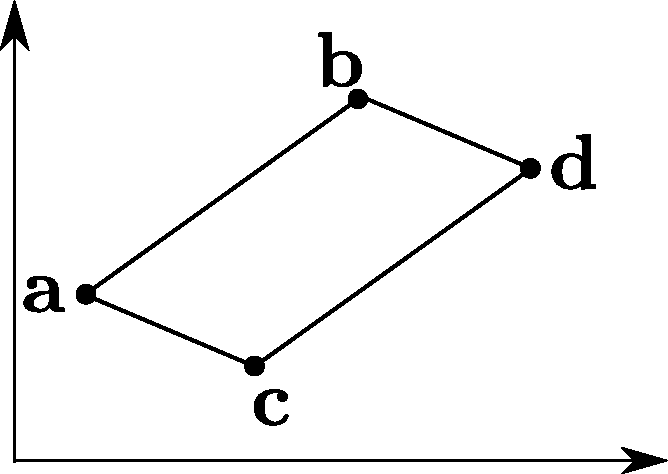
\includegraphics[width=2.5in]{figures/arithmetic_proportion.pdf}
  \caption{$\mathbf{a}, \mathbf{b}, \mathbf{c}, \mathbf{d}$
  are in arithmetic proportion iff they are the four vertices of a
  parallelogram.}
\label{FIG:arithmetic_proportion}
\end{figure}

Even if they did not state it in these terms, Rumelhart and Abrahamsen (Section
\ref{SEC:rumelhart_Abrahamsen}) clearly used the arithmetic proportion for their model of
analogical reasoning.

We have seen that in $\mathbb{B}$, and thus in $\mathbb{B}^m$, the Boolean
proportion and the arithmetic proportion are equivalent. This means that a
proportion in $\mathbb{B}^m$ can also be represented as a (potentially
\textit{flat}) parallelogram.
Figure \ref{FIG:proportions_in_B2} illustrates the proportions that one can
build in $\mathbb{B}^2$:
\begin{itemize}
  \item the proportion $\mathbf{a}: \mathbf{b} :: \mathbf{c} : \mathbf{d}$ and
    its 7 other equivalent forms, making up the parallelogram
    $\mathbf{a}\mathbf{b}\mathbf{c}\mathbf{d}$ ;
  \item the proportions that we can build using any pair of vertices, for
    example $\mathbf{a} : \mathbf{d} :: \mathbf{a} : \mathbf{d}$. Each of these
    proportions has three other equivalent forms: in our case $\mathbf{a} :
    \mathbf{a} :: \mathbf{d} : \mathbf{d}$, $\mathbf{d} : \mathbf{a} ::
    \mathbf{d} : \mathbf{a}$ and $\mathbf{d} : \mathbf{d} :: \mathbf{a} :
    \mathbf{a}$ ;
  \item the four proportions involving each vertex independently, for example
    $\mathbf{b}:\mathbf{b}::\mathbf{b}:\mathbf{b}$.
\end{itemize}

\begin{figure}[!h]
\centering
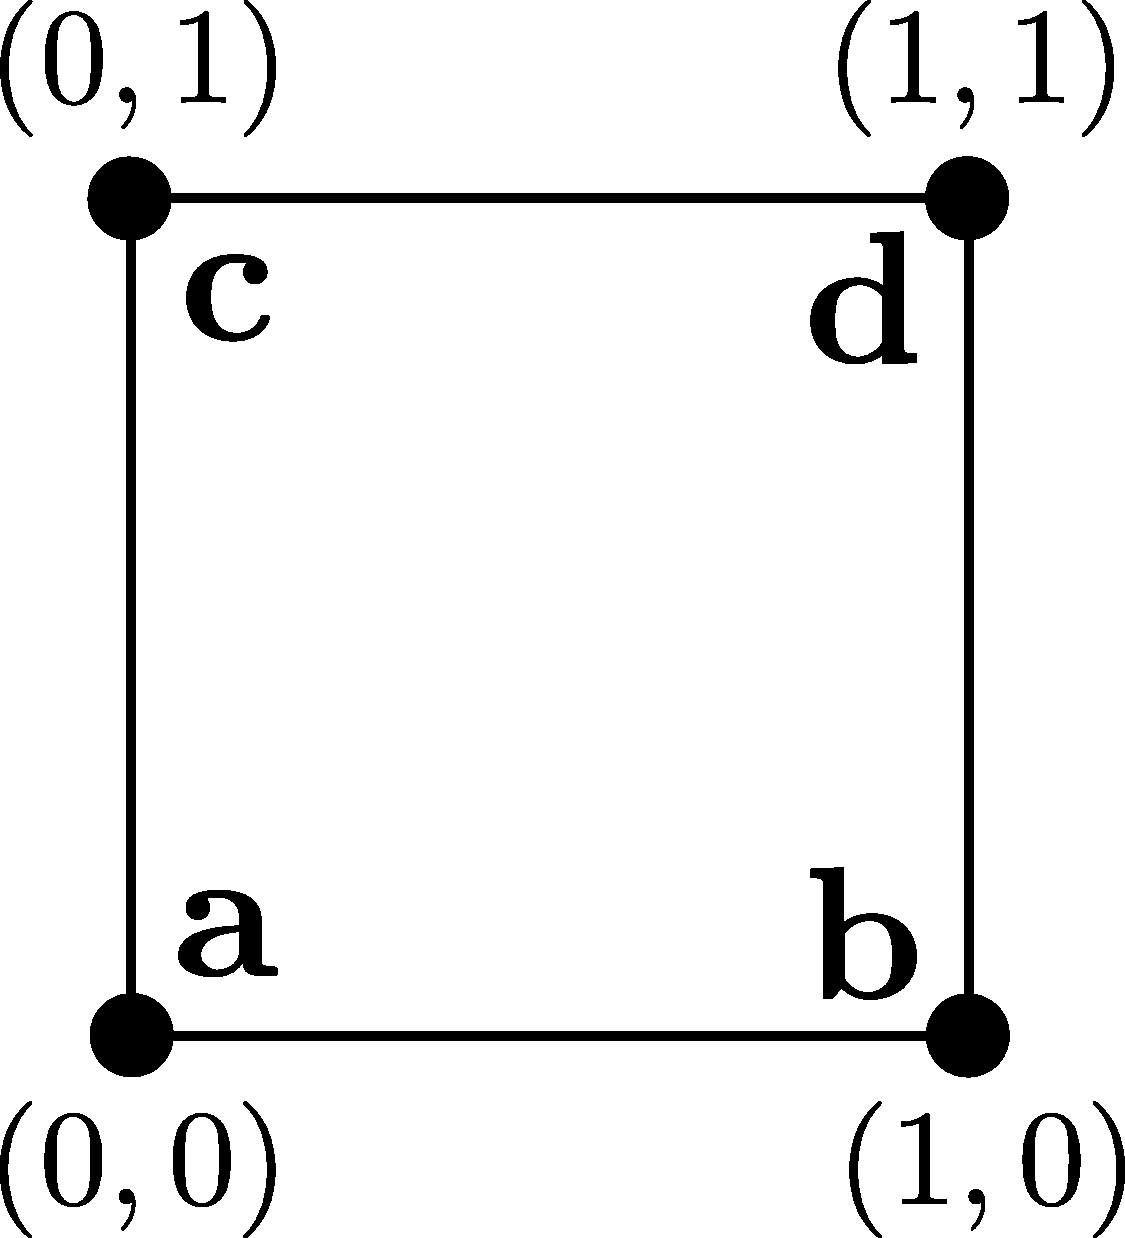
\includegraphics[width=1.5in]{figures/proportions_in_B2.pdf}
  \caption{The $36$ proportions in $\mathbb{B}^2$.}
\label{FIG:proportions_in_B2}
\end{figure}

All in all, this makes up to $36 = 8 + 6 \times 4 + 4$ proportions, but only $1
+ 6 + 4 = 11$ of them can be considered \textit{unique} (up to equivalence) and
only one is non-flat\footnote{\textit{flat} proportion are those that make up
flat parallelograms. This naming convention is actually fortunate, because
these proportion are in practice absolutely useless, as it will soon become
clear.}. In section \ref{SEC:number_of_parallelograms_in_Bm}, we will further
investigate the number of unique proportions that can be built in
$\mathbb{B}^m$.

Going a dimension further can still be insightful. Figure \ref{FIG:cubes_in_B3}
illustrates the 12 non-flat proportions that exist in $\mathbb{B}^3$. These
proportions are the parallelograms making up the 6 faces of the $3$-cube, and
six other \textit{diagonal} parallelograms. The flat proportions are not (all)
shown for the sake of clarity.

\begin{figure}[!h]
\centering
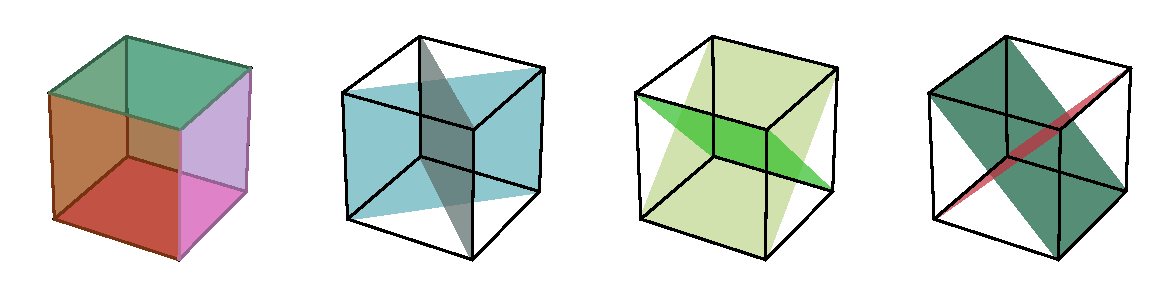
\includegraphics[width=\linewidth]{figures/cubes_in_B3.pdf}
  \caption{The twelve \textit{non-flat} parallelograms in $\mathbb{B}^3$.}
\label{FIG:cubes_in_B3}
\end{figure}

Before applying our fresh knowledge to a classification problem in the next
section, let us first note the following remarkable property, which will be
useful to us much later in Section \ref{TODO}:

\begin{property}
  \label{PROPER:hamming_distance_boolean_proportion}
  Let $\mathbf{a}, \mathbf{b},\mathbf{c}, \mathbf{d}$ in $\mathbb{B}^m$, and
  let $H(\mathbf{x}, \mathbf{x'})$ be the Hamming distance between $\mathbf{x}$
  and $\mathbf{x'}$, i.e. the number of components we need to flip to transform
  $\mathbf{x}$ into $\mathbf{x'}$ (or the reverse).\\
  If $\mathbf{a} : \mathbf{b}
  :: \mathbf{c} : \mathbf{d}$, then these three equalities hold:

  $$
  \begin{cases}
    H(\mathbf{a}, \mathbf{b}) = H(\mathbf{c}, \mathbf{d})\\
    H(\mathbf{a}, \mathbf{c}) = H(\mathbf{b}, \mathbf{d})\\
    H(\mathbf{a}, \mathbf{d}) = H(\mathbf{b}, \mathbf{c}).
  \end{cases}
  $$
\end{property}

We can easily verify this property in $\mathbb{B}$ from Table
\ref{TAB:six_valid_patterns}. The general case in $\mathbb{B}^m$ immediately
follows from Definition \ref{DEF:analogy_for_vectors}. Sadly, Property
\ref{PROPER:hamming_distance_boolean_proportion} only offers a necessary
condition for a proportion to hold, and not a sufficient one. We note that
while the first two properties $H(\mathbf{a}, \mathbf{b}) = H(\mathbf{c},
\mathbf{d})$ and $H(\mathbf{a}, \mathbf{c}) = H(\mathbf{b}, \mathbf{d})$ are
classical properties for parallelograms, the third one $H(\mathbf{a},
\mathbf{d}) = H(\mathbf{b}, \mathbf{c})$ is only true for rectangles. In fact,
the parallelograms that we can build in $\mathbb{B}^m$ are always rectangles.

\section{Machine learning with Boolean proportions: a quick walk-through}
\label{SEC:machine_learning_with_boolean_proportions}

We now have enough background on Boolean proportions to start doing some machine
learning. Here is our problem. We consider the set $\mathbb{B}^m$ and its $2^m$
elements. For various $\mathbf{x} \in \mathbb{B}^m$, we know the value of
$f(\mathbf{x})$, where $f$ is a function from $\mathbb{B}^m$ to $\mathbb{B}$.
The value $f(\mathbf{x})$ is called the \textbf{class} of $\mathbf{x}$, or its
\textbf{label}. The set $S \subsetneq \mathbb{B}^m$ of elements for which
$f(\mathbf{x})$ is known is called the \textbf{training set}. For any element
$\mathbf{x} \notin S$, $f(\mathbf{x})$ is unknown and our goal is to guess it:
this is a binary \textbf{classification problem}.

Suppose we're in $\mathbb{B}^3$ and consider Figure
\ref{FIG:classification_problem}.
\begin{figure}[!h]
\centering
  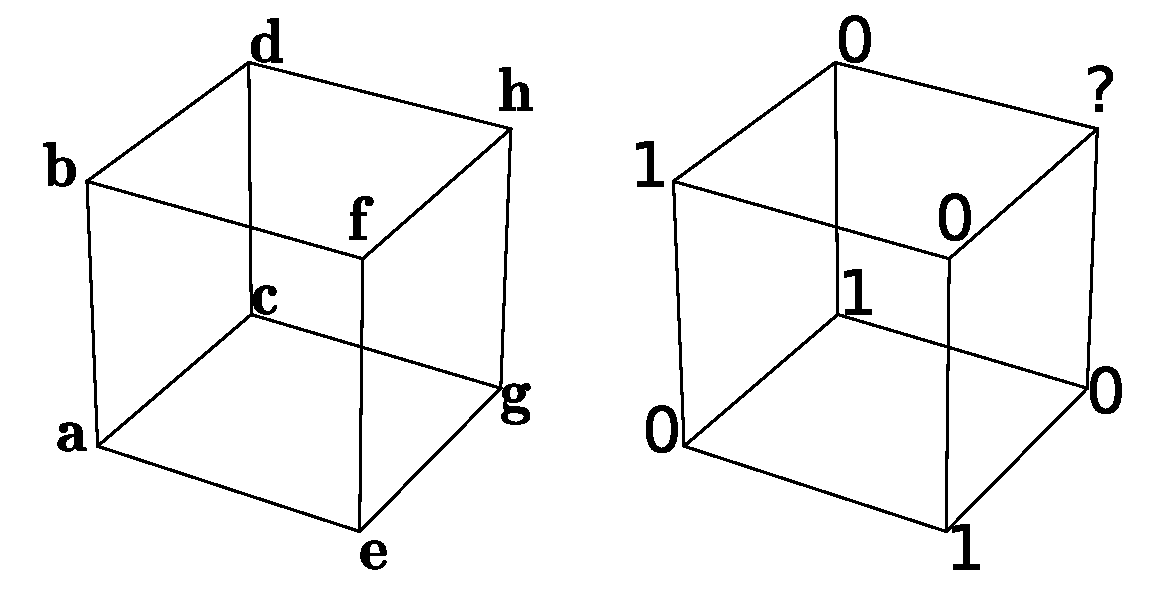
\includegraphics[width=3in]{figures/classification_problem.pdf}
  \caption{A classification problem in $\mathbb{B}^3$. Labels $f(\mathbf{x})$
  are on the right cube.}
\label{FIG:classification_problem}
\end{figure}
We know the values of $f(\mathbf{x})$ for
every single element $\mathbf{x}$ but $\mathbf{h}$, so $S = \{ \mathbf{a}, \mathbf{b},
\mathbf{c}, \mathbf{d}, \mathbf{e}, \mathbf{f}, \mathbf{g}\}$. To guess the
value of $f(\mathbf{h})$, we will use the so-called \textbf{analogical
inference principle}, which states that if four elements $\mathbf{a},
\mathbf{b}, \mathbf{c}, \mathbf{d}$ are in proportion, then their class should
also be in proportion:
$$
\infer{f(\mathbf{a}) : f(\mathbf{b}) :: f(\mathbf{c})
: f(\mathbf{d})}{\mathbf{a} : \mathbf{b} :: \mathbf{c} : \mathbf{d}}
$$

This is obviously an unsound principle, in that the conclusion does not
logically follows from the premise. But as we will see in this document, it can
still be useful.

As we want to guess the value of $f(\mathbf{h})$, this principle leads us to
look for all 3-tuples $(\mathbf{x}, \mathbf{y}, \mathbf{z}) \in S^3$ such that
$\mathbf{x}:\mathbf{y}::\mathbf{z}:\mathbf{h}$.  The analogical inference then
states that we should have
$f(\mathbf{x}):f(\mathbf{y})::f(\mathbf{z}):f(\mathbf{h})$. Figure
\ref{FIG:cubes_in_B3} tells us that there are 6 (non-flat) parallelograms
involving $\mathbf{h}$ as a vertex. The six unique corresponding proportions
are:

\begin{enumerate}
  \item $\mathbf{a} : \mathbf{b} :: \mathbf{g} : \mathbf{h}$
  \item $\mathbf{a} : \mathbf{d} :: \mathbf{e} : \mathbf{h}$
  \item $\mathbf{a} : \mathbf{c} :: \mathbf{f} : \mathbf{h}$
  \item $\mathbf{b} : \mathbf{d} :: \mathbf{f} : \mathbf{h}$
  \item $\mathbf{e} : \mathbf{f} :: \mathbf{g} : \mathbf{h}$
  \item $\mathbf{c} : \mathbf{g} :: \mathbf{d} : \mathbf{h}$
\end{enumerate}

Applying the analogical inference principle to the first proportion $\mathbf{a}
: \mathbf{b} :: \mathbf{g} : \mathbf{h}$ leads to $f(\mathbf{a}) :
f(\mathbf{b}) :: f(\mathbf{g}) : f(\mathbf{h})$, which is equivalent to:
$$0:1::0:f(\mathbf{h}).$$ By referring to Table \ref{TAB:six_valid_patterns}, we
notice that $f(\mathbf{h})$ should be equal to $1$ for the proportion
$f(\mathbf{a}) : f(\mathbf{b}) :: f(\mathbf{g}) : f(\mathbf{h})$ to be a valid
one, because $0:1::0:1$. So we keep $1$ in the back of our head as a possible
candidate for $f(\mathbf{h})$: we say that $1$ is a \textbf{candidate
solution} for $f(\mathbf{h})$.

What we have just done is the \textbf{solving of an analogical equation}.
Generally speaking, an analogical equation is a proportion $a:b::c:x$ in a
context where $x$ is unknown. Determining the value of $x$ is then called the
\textit{solving} of this equation. Depending on the nature and values of $a, b$,
and $c$, there may or may not exist a solution, and it might not be unique. In a
Boolean setting, an equation is solvable for 6 patterns of $a, b, c$ (the 6
patterns of Table \ref{TAB:six_valid_patterns}, naturally). As we can see, the
solution is always unique:

\begin{proposition}
  \label{PROPOS:equation_solving}
  Let $a, b, c$ in $\mathbb{B}$. The analogical equation
  $a :b::c:x$
  is solvable if and only if $a = b$ or $a = c$. The solution denoted
  $\emph{sol}(a, b, c)$ is then given by:
  $$
  \begin{cases}
    \emph{sol}(a, b, c) \eqdef c \emph{ if } a = b,\\
    \emph{sol}(a, b, c) \eqdef b \emph{ if } a = c,
  \end{cases}
  $$
  or more generally:
  $$\emph{sol}(a, b, c) \eqdef c - a + b,$$
  because the Boolean proportion is a particular case of the arithmetic
  proportion.
\end{proposition}

Let's get back to the estimation of $f(\mathbf{h})$. Applying the analogical
inference principle to the second proportion $\mathbf{a} : \mathbf{d} ::
\mathbf{e} : \mathbf{h}$ leads $f(\mathbf{a)} : f(\mathbf{d}) :: f(\mathbf{e})
: f(\mathbf{h})$, and to the solving of $0:0::1:f(\mathbf{h})$. Here again, the
solution is $1$, just like the candidate of the first proportion.
The third proportion  $\mathbf{a} : \mathbf{c} :: \mathbf{f} : \mathbf{h}$
leads to the solving of $0:1::0:f(\mathbf{h})$, also claiming that $1$ is a good candidate.

And now the fourth proportion $\mathbf{b} : \mathbf{d} :: \mathbf{f} :
\mathbf{h}$, which leads to $1:0::0:f(\mathbf{h})$. \textbf{This equation is not
solvable}: neither $1:0::0:1$ nor $1:0::0:0$ are valid proportions. We thus
simply discard the proportion $\mathbf{b} : \mathbf{d} :: \mathbf{f} :
\mathbf{h}$ as a potential source of information about $f(\mathbf{h)}$, because
we are not in a position to apply the analogical inference principle. We can
easily verify that the fifth and sixth (and last!) proportions also lead to
non-solvable equations.

All in all, we are left with three candidates coming from the first three
proportions, all of which are equal to $1$. Our guess will thus be that
$f(\mathbf{h})$ should be equal to $1$. Is this correct? Well in real-world
settings, there is no way to know for sure, because the ground truth function
$f$ is unknown (otherwise, there is no point in trying to classify $\mathbf{h}$
in the first place). The undeniable perks of artificial examples is that we can
do how we please, and define the function $f$ by
$$\forall \mathbf{x}, ~ f(\mathbf{x}) = f(x_1, x_2, x_3) = x_1 \oplus x_2 \oplus x_3,$$
where $\oplus$ denotes the XOR operator, which is both commutative and
associative: $a \oplus b = (a \wedge \neg b) \vee (\neg a \wedge b)$. So in our
case, yes, the true value of $f(\mathbf{h})$ is indeed $1$ and our prediction
is correct.

Notice that we have so far lightheartedly ignored  all the flat proportions.
This is because none of these proportions allow us to derive a solvable
equation. Considering for example $\mathbf{d} : \mathbf{h} :: \mathbf{d} :
\mathbf{h}$, we're led to the solving of $f(\mathbf{d}) : f(\mathbf{h}) ::
f(\mathbf{d}) : f(\mathbf{h})$, or equivalently of $0 : f(\mathbf{h}) :: 0 :
f(\mathbf{h})$. Both values $0$ and $1$ could lead to equally valid proportions
here, so there is simply no predictive power in the flat proportions. We have
also only considered unique proportions, up to equivalence. The first proportion
$\mathbf{a} : \mathbf{b} :: \mathbf{g} : \mathbf{h}$ for example is equivalent
to $\mathbf{a} : \mathbf{g} :: \mathbf{b} : \mathbf{h}$ (using central
permutation), which we could have
used instead. As any two equivalent proportions lead to the same solution for
their associated class equations, we usually choose to ignore all other equivalent
proportions, which allows to divide the number of equation solving by a factor
of $2$.

Here is a small outline of our classification process, that was entirely
governed by the analogical inference principle. Our goal was to guess the value
of $f(\mathbf{h})$:

\begin{itemize}
  \item We first looked at all the $(\mathbf{x}, \mathbf{y}, \mathbf{z}) \in
    \mathbf{B}^3$ such that:
    \begin{itemize}
      \item $f(\mathbf{x}), f(\mathbf{y})$ and $f(\mathbf{z})$ are known ;
      \item $\mathbf{x}:\mathbf{y}::\mathbf{z}:\mathbf{h}$ holds ;
      \item the \textbf{class equation} $f(\mathbf{x}) :f(\mathbf{y}) ::
        f(\mathbf{z}) :s$ is \textbf{solvable}. $s$ is called a
        \textbf{candidate solution}.
    \end{itemize}
    Each of our three candidate solutions $s_1, s_2, s_3$ agreed on the same prediction:
    $s_i = 1$ for all $i$.
  \item We thus estimated that $f(\mathbf{h})$ should indeed be equal to $1$.
\end{itemize}

This minimal example of analogical classification raises a few concerns, which
we will be thoroughly addressed in this document:
\begin{enumerate}
  \item All of the three candidate solutions for $f(\mathbf{h})$ agreed on the
    same prediction: $1$. What if one of them predicted $0$? A first drastic
    option is to refuse to classify $\mathbf{h}$, on the basis that if the
    candidates cannot agree on their predictions, then we should not trust any
    of them. As it will become clear, in practice the candidates never really
    completely agree, even though sometimes a clear majority emerges. So this
    strategy would make the prediction impossible for most elements $\mathbf{x}
    \notin S$. A wiser option is to consider an aggregation of the candidate
    solutions: the most common one, for example. This is the option that has
    been took on so far, as we will see in the next chapter.
  \item Here, by chance, the set of candidate solutions for $f(\mathbf{h})$ was
    not empty: we found three candidate solutions. What happens if we can't
    find any candidate? This case arises when there are no 3-tuple
    $(\mathbf{x}, \mathbf{y}, \mathbf{z}) \in S^3$ such that $\mathbf{x} :
    \mathbf{y}::\mathbf{z}:\mathbf{h}$ and such that the associated equation
    $f(\mathbf{x}):f(\mathbf{y})::f(\mathbf{z}):f(\mathbf{h})$ is solvable. In
    the works of Stroppa and Yvon (\cite{StrYvoCNLL05}), such an $\mathbf{h}$
    cannot be classified. The notion of \textbf{analogical dissimilarity}
    as used in \cite{BayMicDelIJCAI07} will allow to bypass this issue. One of
    the contribution of our work is to provide a unifying view of the two
    techniques, and is the purpose of Chapter \ref{CHAP:functional_definition}.

  \item How \textit{safe} is the analogical inference principle? What are some
    theoretical guarantees that could allow us to use it on a sound basis? This
    question stays, to this day, unanswered. In Chapter \ref{TODO} however, we
    will provide a complete characterization of the Boolean functions $f$ that
    allow to derive sound conclusions.
\end{enumerate}

\paragraph{How many proportions can we build in $\mathbb{B}^m$?\\}
\label{SEC:number_of_parallelograms_in_Bm}

Exactly $6^m$! And it is fairly easy to derive: there are $6$ proportions in
$\mathbb{B}$. As a proportion in $\mathbb{B}^2$ is the concatenation of any two
proportions in $\mathbb{B}$, there are exactly $6^2 = 36$ proportions in
$\mathbb{B}^2$, as seen in Section
\ref{SEC:shortcut_from_aristotle_to_boolean_proportions}. Analogical
proportions in $\mathbb{B}^m$ are defined component-wise, i.e. they are the
concatenation of $m$ proportions in $\mathbb{B}$. Equivalently, a proportion in
$\mathbb{B}^m$ is the concatenation of a proportion in $\mathbb{B}^{m - 1}$ and
a proportion in $\mathbb{B}$. By trivial induction, we can build $6^m$
proportions in $\mathbb{B}^m$.

But let's now ask a more relevant and challenging question: how many
\textit{useful} proportions can we build in $\mathbb{B}^m$? By \textit{useful},
we mean proportions that could be used for classification purposes.

\begin{aquote}{The astute reader, who has been struck by divine light}
  What a silly question! There are obviously $\frac{6^m}{8} - 4^{m - 1} + 2^{m
  - 3}$ such proportions! How can you not be aware of the A016283 sequence from
  the OEIS\footnote{The On-line Encyclopedia of Integer Sequences
  (http://oeis.org/A016283)}?!
\end{aquote}

Unfortunately, we, who have not (yet) been struck by divine light, will have to
derive this formula ourselves. We have seen in Section \ref{TODO} that the only
proportions $\mathbf{a} : \mathbf{b} :: \mathbf{c} : \mathbf{d}$ that are
useful for classification purposes are those where all elements $\mathbf{a},
\mathbf{b}, \mathbf{c}, \mathbf{d}$ are distinct. We thus want to exclude from
the $6^m$ proportions those that comply with one of the following patterns:

\begin{itemize}
  \item $\mathbf{a}: \mathbf{a} :: \mathbf{a} : \mathbf{a}$
  \item $\mathbf{a}: \mathbf{b} :: \mathbf{a} : \mathbf{b}$, and its three
    equivalent forms $\mathbf{a}: \mathbf{a} :: \mathbf{b} : \mathbf{b}$,
    $\mathbf{b}: \mathbf{a} :: \mathbf{b} : \mathbf{a}$, and $\mathbf{b}:
    \mathbf{b} :: \mathbf{a} : \mathbf{a}$
\end{itemize}

Now, let's count them.

\begin{itemize}
  \item Each of the $2^m$ vertex $\mathbf{a}$ will generate a proportion of the
    form $\mathbf{a}: \mathbf{a} :: \mathbf{a} : \mathbf{a}$, so there are
    exactly $2^m$ proportions of this kind.
  \item Every pair $(\mathbf{a}, \mathbf{b})$ of vertices will generate four
    proportions:
    \begin{itemize}
      \item $\mathbf{a}: \mathbf{b} :: \mathbf{a} : \mathbf{b}$,
      \item $\mathbf{a}: \mathbf{a} :: \mathbf{b} : \mathbf{b}$,
      \item $\mathbf{b}: \mathbf{a} :: \mathbf{b} : \mathbf{a}$,
      \item $\mathbf{b}: \mathbf{b} :: \mathbf{a} : \mathbf{a}$.
    \end{itemize}
    There are $\binom{2^m}{2}$ distinct pairs of vertices, so in total this
    makes $4\cdot \binom{2^m}{2}$ proportions of the form $\mathbf{a}: \mathbf{b} ::
    \mathbf{a} : \mathbf{b}$ with its equivalent forms.
\end{itemize}

We are then left with the number of $6^m - 2^m - 4\cdot\binom{2^m}{2}$ useful
proportions. We know that for each of these proportions, all elements
$\mathbf{a}, \mathbf{b}, \mathbf{c}, \mathbf{d}$  are distinct. For each of
them, there are thus 7 other equivalent forms, which reduces the number of
useful and unique (up to equivalence) proportions to:
$$P_m = \frac{1}{8} \left[6^m - 2^m - 4\cdot\binom{2^m}{2} \right].$$
This is precisely the number of non-flat parallelograms in an $m$-dimensional
cube. The A016283 sequence of the OEIS mentioned above actually describes
\textit{the number of rectangles that can be formed from the vertices of an
$m$-dimensional cube}, which is exactly equivalent. Using
the fact that $\binom{n}{k} = \frac{n}{k}\binom{n - 1}{k - 1}$, it can be shown
that the two formulas $\frac{1}{8} \left[6^m - 2^m - 4\cdot\binom{2^m}{2} \right]$
and $\frac{6^m}{8} - 4^{m - 1} + 2^{m- 3}$ are, fortunately, the same.

To be fair, we have no idea how the formula of the OEIS was derived, but we
firmly believe that ours is the most entertaining one. Table
\ref{TAB:n_params_in_cube} gives the values of $P_m$ for the first $10$ values
of $m$.
\begin{table}[h!]
\centering
  \begin{tabular}{ l  l }
\toprule
 $m$ & $P_m$\\
\midrule
    1	&	0\\
    2 &	1\\
    3	&	12\\
    4	&	100\\
    5 &	720\\
    6 &	4816\\
    7 &	30912\\
    8 &	193600\\
    9 & 1194240\\
    10 & 7296256\\
\bottomrule
\end{tabular}
\caption{Number of unique non-flat proportions in an $m$-dimensional cube.}
\label{TAB:n_params_in_cube}
\end{table}
Naturally, $P_2$ and $P_3$ are in accordance with our empirical  results from
Figures \ref{FIG:proportions_in_B2} and \ref{FIG:cubes_in_B3}. The fact that
$P_1 = 0$ means that no inference can be done with analogical proportion in
$\mathbb{B}$, which is perfectly normal: in $\mathbb{B}$, all proportions are
flat (i.e. the pattern is always $a:b::a:b$ or $a:a::b:b$).

\section{Formal definitions}
\label{SEC:formal_definitions_proportions}

The Boolean proportion was introduced in the previous section in an informal
way, along with many key concepts such as the solving on an analogical
equation, and the analogical inference principle. In this section, we will
provide the definition of the Boolean proportion (and others) in a more formal
way.

Probably the first use of formal proportions is that of Lepage in
\cite{Lep04} who, starting from the three aforementioned axioms, formally
defined analogical proportions over alphabets of letters with the aim of
generating (analogical) formal languages. His definition have later been
generalized in the works of Stroppa and Yvon (see \cite{StrYvoCNLL05} and
\cite{StrYvoREPORT05})\footnote{In the same work, Stroppa and Yvon also laid
the foundations of analogical learning as used in this thesis (see Section
\ref{la section})}, who provided an algebraic factorization-based definition of
analogical proportions in semigroups:

\begin{definition}
\label{DEF:proportion_semi_group}
Let $(U, \oplus)$ be a semigroup, i.e. $U$ is a set and $\oplus$ is an
  associative binary operation. Four elements $a, b, c, d \in U$, are in proportion if
  there exist some factorization
  \begin{align*}
    a &= a_1 \oplus a_2 \oplus \cdots \oplus a_n\\
    b &= b_1 \oplus b_2 \oplus \cdots \oplus b_n\\
    c &= c_1 \oplus c_2 \oplus \cdots \oplus c_n\\
    d &= d_1 \oplus d_2 \oplus \cdots \oplus d_n,
  \end{align*}

  such that for all $i \in [1, n]$, 
  $$
  \begin{cases}
    a_i = b_i \emph{ and } c_i = d_i\\
    \emph{or}\\
    a_i = c_i \emph{ and } b_i = d_i.
  \end{cases}
  $$
\end{definition}

We can clearly foresee here the features of the Boolean proportion. It will be
insightful to instantiate $U$ as the set of natural number $\mathbb{N}$ and
$\oplus$ as the usual multiplication $\times$. In this setting, let's consider
the prime factorization of:

\begin{align*}
  a &= 30 = 1 \times 2 \times 3 \times 5\\
  b &= 60 = 2 \times 2 \times 3 \times 5\\
  c &= 25 = 1 \times 1 \times 5 \times 5\\
  d &= 50 = 2 \times 1 \times 5 \times 5
\end{align*}

For each $i$, we either have $a_i = b_i$ and $c_i = d_i$ ($i = 2, 3, 4$) or
$a_i = c_i$ and $b_i = d_i$ ($i = 1, 4$). We can then say that $a, b, c, d$ are
in proportion, i.e. $30: 60 :: 25:50$. Naturally, the reader will recognize
here the geometric proportion: $\frac{30}{60} = \frac{25}{50}$.
Starting from this general definition, other proportions have been defined in
various domains, namely analogies between trees, lattices, or matrices
\cite{MicDel04, StrYvoREPORT05, MicBayDelJAIR08}. However, we will not detail
them further here and rather focus on other domains of interest.

In \cite{Lep03}, Lepage defines an analogy between sets as follows: four subsets
$A, B, C, D$ of a universal set $X$ are in proportion if $A$ can be transformed
into $B$ by adding and deleting the same elements as to transform $C$ into $D$.
A more formal definition has been given in \cite{StrYvoREPORT05}:

\begin{definition}
  \label{DEF:analogy_set_facto}
  Let $A, B, C, D \subset X$. $A, B, C, D$ are in proportion if there exists
  four subsets $U, V, W$ and $Z$ (not necessarily disjoint) such that:
  $$
  \begin{cases}
    A = U \cup V\\
    B = U \cup W\\
    C = Z \cup V\\
    D = Z \cup W\\
  \end{cases}
  $$
\end{definition}

To go from $A$ to $B$, one needs to add $W$ and remove $V$. To go from $C$ to
$D$, one needs to do the exact same thing: add $W$ and remove $V$. An
equivalent definition has been given in \cite{MicPra09}:

\begin{definition}
  \label{DEF:analogy_set_miclet_henri}
  Let $A, B, C, D \subset X$. $A, B, C, D$ are in proportion if:
  $$
  A \setminus B = C \setminus D \emph{ and } B \setminus A = D \setminus A
  $$
\end{definition}

Definition \ref{DEF:analogy_set_miclet_henri} reads as \textit{$A$ differs from
$B$ as $C$ differs from $D$, and $B$ differs from $A$ as $D$ differs from $C$},
which is naturally equivalent to the statement of Definition
\ref{DEF:analogy_set_facto}: $A \setminus B = C \setminus D = V$, and $B
\setminus A = D \setminus A  = W$. The formula of Definition
\ref{DEF:analogy_set_miclet_henri} is actually equivalent to the following form
(not without using various ingenious tweaks): $$A \cup D = B \cup C \text{ and
} A \cap D = B \cap C.$$

As an example, let's consider $A = \{a, b, c, g\}, B = \{a, b, d, e, g\}, C =
\{c, f, g\}$ and $D = \{d, e, f, g\}$, as summed-up in Table
\ref{TAB:analogy_sets}.

\begin{table}[h!]
\centering
$$
\begin{tabular}{ c  c  c  c  c  c  c  c }
\toprule
  & a & b & c & d & e & f & g\\
\midrule
  A & \times & \times & \times &  &  &  & \times \\
  B & \times & \times &  & \times & \times &  & \times\\
  C &  &  & \times &  &  & \times & \times\\
  D &  &  &  & \times & \times & \times & \times\\
\bottomrule
\end{tabular}
$$
\caption{Four sets $A, B, C, D$ in analogical proportion.}
\label{TAB:analogy_sets}
\end{table}

Setting $U = \{a, b, g\}, V = \{c\}, W = \{d, e\}$ and $Z = \{f, g\}$, the
conditions of Definition  \ref{DEF:analogy_set_facto}  are clearly satisfied.
Also, $A \setminus B = C \setminus D = \{c\} = V$, and $B\setminus A = D
\setminus C = \{d, e\} = W$. Finally, $A \cup D = B \cup C = \{a, b, c, d, e,
f, g\}$ and $A\cap D = B\cap C = \{g\}$.

We can also recognize in Table \ref{TAB:analogy_sets} that the conditions of
Definition \ref{DEF:proportion_semi_group} are satisfied, i.e. for all $i$ we
have either $A_i = B_i$ and $C_i = D_i$, or $A_i = C_i$ and $B_i = D_i$.

The definition of the Boolean proportion can be directly derived from
Definition \ref{DEF:analogy_set_miclet_henri} and by considering the set
$\mathbb{B} = \{0, 1\}$:

\begin{definition}
  \label{DEF:boolean_proportion}
  Four elements $a, b, c, d$ in $\mathbb{B} = \{0, 1\}$ are in proportion if
  \begin{alignat*}{2}
    &(a \leftrightarrow b \wedge c \leftrightarrow d) && \vee (a
    \leftrightarrow c \wedge b \leftrightarrow d), \emph{ or equivalently}\\
     & (a \wedge d \leftrightarrow b \wedge c) &&\wedge (a \vee  d
    \leftrightarrow b \vee c),
  \end{alignat*}
  where $\leftrightarrow$ stands for the equivalence connective.
\end{definition}

These scary formulas state the exact same facts as the previous definition,
i.e. that $a$ differs from $b$ as $c$ differs from $d$ and conversely $b$
differs from $a$ as $d$ differs from $c$. Naturally, Definition
\ref{DEF:boolean_proportion} and \ref{DEF:boolean_proportion_informal} (the one
we initially suggested) are equivalent.

We now have to go back to the 80's and mention the pioneering work of Sheldon
Klein, who, to some extent, defined his \textit{own} Boolean analogical
proportion. His definition states that $a, b, c, d$ in $\mathbb{B}$ are in
proportion if $a \oplus b = c \oplus d$, where $\oplus$ is the XOR operator.
This definition, less restrictive than Definition \ref{DEF:boolean_proportion},
amounts to adding two new patterns to Table \ref{TAB:six_valid_patterns}:
$0:1::1:0$, and its counterpart $1:0::0:1$. These two patterns seem appealing at
first sight, because they capture the fact that $a : \neg a :: b \neg b$.
However, they lead to the fact that $a:b::c:d$ if and only if $b : a :: c :d$,
which seems quite unnatural for an analogy. In Section \ref{TODO}, we will show
that the two definitions of Boolean proportion (the standard one of Definition
\ref{DEF:boolean_proportion} and that of Klein) share common properties with
regard to their suitability with the analogical inference principle. We will
also see that in spite of this, the standard model seems to be the most useful
one in practice.

The notion of Boolean analogical proportion has recently been extended to the
concept of \textbf{logical proportion} (see e.g. \cite{PraRic14}), but their
details are out of the scope of this document.
